\documentclass[1p]{elsarticle_modified}
%\bibliographystyle{elsarticle-num}

%\usepackage[colorlinks]{hyperref}
%\usepackage{abbrmath_seonhwa} %\Abb, \Ascr, \Acal ,\Abf, \Afrak
\usepackage{amsfonts}
\usepackage{amssymb}
\usepackage{amsmath}
\usepackage{amsthm}
\usepackage{scalefnt}
\usepackage{amsbsy}
\usepackage{kotex}
\usepackage{caption}
\usepackage{subfig}
\usepackage{color}
\usepackage{graphicx}
\usepackage{xcolor} %% white, black, red, green, blue, cyan, magenta, yellow
\usepackage{float}
\usepackage{setspace}
\usepackage{hyperref}

\usepackage{tikz}
\usetikzlibrary{arrows}

\usepackage{multirow}
\usepackage{array} % fixed length table
\usepackage{hhline}

%%%%%%%%%%%%%%%%%%%%%
\makeatletter
\renewcommand*\env@matrix[1][\arraystretch]{%
	\edef\arraystretch{#1}%
	\hskip -\arraycolsep
	\let\@ifnextchar\new@ifnextchar
	\array{*\c@MaxMatrixCols c}}
\makeatother %https://tex.stackexchange.com/questions/14071/how-can-i-increase-the-line-spacing-in-a-matrix
%%%%%%%%%%%%%%%

\usepackage[normalem]{ulem}

\newcommand{\msout}[1]{\ifmmode\text{\sout{\ensuremath{#1}}}\else\sout{#1}\fi}
%SOURCE: \msout is \stkout macro in https://tex.stackexchange.com/questions/20609/strikeout-in-math-mode

\newcommand{\cancel}[1]{
	\ifmmode
	{\color{red}\msout{#1}}
	\else
	{\color{red}\sout{#1}}
	\fi
}

\newcommand{\add}[1]{
	{\color{blue}\uwave{#1}}
}

\newcommand{\replace}[2]{
	\ifmmode
	{\color{red}\msout{#1}}{\color{blue}\uwave{#2}}
	\else
	{\color{red}\sout{#1}}{\color{blue}\uwave{#2}}
	\fi
}

\newcommand{\Sol}{\mathcal{S}} %segment
\newcommand{\D}{D} %diagram
\newcommand{\A}{\mathcal{A}} %arc


%%%%%%%%%%%%%%%%%%%%%%%%%%%%%5 test

\def\sl{\operatorname{\textup{SL}}(2,\Cbb)}
\def\psl{\operatorname{\textup{PSL}}(2,\Cbb)}
\def\quan{\mkern 1mu \triangleright \mkern 1mu}

\theoremstyle{definition}
\newtheorem{thm}{Theorem}[section]
\newtheorem{prop}[thm]{Proposition}
\newtheorem{lem}[thm]{Lemma}
\newtheorem{ques}[thm]{Question}
\newtheorem{cor}[thm]{Corollary}
\newtheorem{defn}[thm]{Definition}
\newtheorem{exam}[thm]{Example}
\newtheorem{rmk}[thm]{Remark}
\newtheorem{alg}[thm]{Algorithm}

\newcommand{\I}{\sqrt{-1}}
\begin{document}

%\begin{frontmatter}
%
%\title{Boundary parabolic representations of knots up to 8 crossings}
%
%%% Group authors per affiliation:
%\author{Yunhi Cho} 
%\address{Department of Mathematics, University of Seoul, Seoul, Korea}
%\ead{yhcho@uos.ac.kr}
%
%
%\author{Seonhwa Kim} %\fnref{s_kim}}
%\address{Center for Geometry and Physics, Institute for Basic Science, Pohang, 37673, Korea}
%\ead{ryeona17@ibs.re.kr}
%
%\author{Hyuk Kim}
%\address{Department of Mathematical Sciences, Seoul National University, Seoul 08826, Korea}
%\ead{hyukkim@snu.ac.kr}
%
%\author{Seokbeom Yoon}
%\address{Department of Mathematical Sciences, Seoul National University, Seoul, 08826,  Korea}
%\ead{sbyoon15@snu.ac.kr}
%
%\begin{abstract}
%We find all boundary parabolic representation of knots up to 8 crossings.
%
%\end{abstract}
%\begin{keyword}
%    \MSC[2010] 57M25 
%\end{keyword}
%
%\end{frontmatter}

%\linenumbers
%\tableofcontents
%
\newcommand\colored[1]{\textcolor{white}{\rule[-0.35ex]{0.8em}{1.4ex}}\kern-0.8em\color{red} #1}%
%\newcommand\colored[1]{\textcolor{white}{ #1}\kern-2.17ex	\textcolor{white}{ #1}\kern-1.81ex	\textcolor{white}{ #1}\kern-2.15ex\color{red}#1	}

{\Large $\underline{12a_{0094}~(K12a_{0094})}$}

\setlength{\tabcolsep}{10pt}
\renewcommand{\arraystretch}{1.6}
\vspace{1cm}\begin{tabular}{m{100pt}>{\centering\arraybackslash}m{274pt}}
\multirow{5}{120pt}{
	\centering
	\includegraphics[width=112pt]{../../../GIT/diagram.site/Diagrams/png/895_12a_0094.png}\\
\ \ \ A knot diagram\footnotemark}&
\allowdisplaybreaks
\textbf{Linearized knot diagam} \\
\cline{2-2}
 &
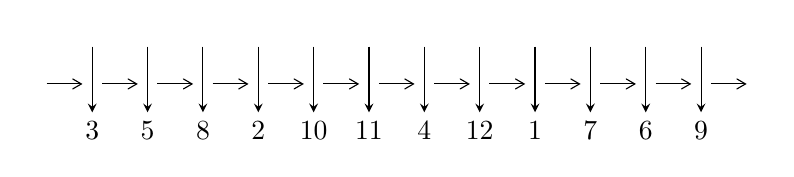
\begin{tikzpicture}[x=20pt, y=17pt]
	% nodes
	\node (C0) at (0, 0) {};
	\node (C1) at (1, 0) {};
	\node (C1U) at (1, +1) {};
	\node (C1D) at (1, -1) {3};

	\node (C2) at (2, 0) {};
	\node (C2U) at (2, +1) {};
	\node (C2D) at (2, -1) {5};

	\node (C3) at (3, 0) {};
	\node (C3U) at (3, +1) {};
	\node (C3D) at (3, -1) {8};

	\node (C4) at (4, 0) {};
	\node (C4U) at (4, +1) {};
	\node (C4D) at (4, -1) {2};

	\node (C5) at (5, 0) {};
	\node (C5U) at (5, +1) {};
	\node (C5D) at (5, -1) {10};

	\node (C6) at (6, 0) {};
	\node (C6U) at (6, +1) {};
	\node (C6D) at (6, -1) {11};

	\node (C7) at (7, 0) {};
	\node (C7U) at (7, +1) {};
	\node (C7D) at (7, -1) {4};

	\node (C8) at (8, 0) {};
	\node (C8U) at (8, +1) {};
	\node (C8D) at (8, -1) {12};

	\node (C9) at (9, 0) {};
	\node (C9U) at (9, +1) {};
	\node (C9D) at (9, -1) {1};

	\node (C10) at (10, 0) {};
	\node (C10U) at (10, +1) {};
	\node (C10D) at (10, -1) {7};

	\node (C11) at (11, 0) {};
	\node (C11U) at (11, +1) {};
	\node (C11D) at (11, -1) {6};

	\node (C12) at (12, 0) {};
	\node (C12U) at (12, +1) {};
	\node (C12D) at (12, -1) {9};
	\node (C13) at (13, 0) {};

	% arrows
	\draw[->,>={angle 60}]
	(C0) edge (C1) (C1) edge (C2) (C2) edge (C3) (C3) edge (C4) (C4) edge (C5) (C5) edge (C6) (C6) edge (C7) (C7) edge (C8) (C8) edge (C9) (C9) edge (C10) (C10) edge (C11) (C11) edge (C12) (C12) edge (C13) ;	\draw[->,>=stealth]
	(C1U) edge (C1D) (C2U) edge (C2D) (C3U) edge (C3D) (C4U) edge (C4D) (C5U) edge (C5D) (C6U) edge (C6D) (C7U) edge (C7D) (C8U) edge (C8D) (C9U) edge (C9D) (C10U) edge (C10D) (C11U) edge (C11D) (C12U) edge (C12D) ;
	\end{tikzpicture} \\
\hhline{~~} \\& 
\textbf{Solving Sequence} \\ \cline{2-2} 
 &
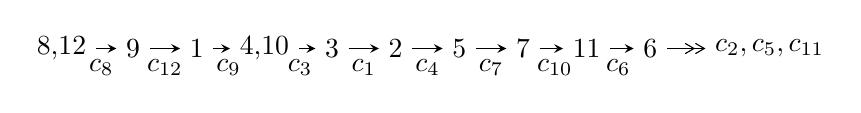
\begin{tikzpicture}[x=23pt, y=7pt]
	% node
	\node (A0) at (-1/8, 0) {8,12};
	\node (A1) at (1, 0) {9};
	\node (A2) at (2, 0) {1};
	\node (A3) at (49/16, 0) {4,10};
	\node (A4) at (33/8, 0) {3};
	\node (A5) at (41/8, 0) {2};
	\node (A6) at (49/8, 0) {5};
	\node (A7) at (57/8, 0) {7};
	\node (A8) at (65/8, 0) {11};
	\node (A9) at (73/8, 0) {6};
	\node (C1) at (1/2, -1) {$c_{8}$};
	\node (C2) at (3/2, -1) {$c_{12}$};
	\node (C3) at (5/2, -1) {$c_{9}$};
	\node (C4) at (29/8, -1) {$c_{3}$};
	\node (C5) at (37/8, -1) {$c_{1}$};
	\node (C6) at (45/8, -1) {$c_{4}$};
	\node (C7) at (53/8, -1) {$c_{7}$};
	\node (C8) at (61/8, -1) {$c_{10}$};
	\node (C9) at (69/8, -1) {$c_{6}$};
	\node (A10) at (11, 0) {$c_{2},c_{5},c_{11}$};

	% edge
	\draw[->,>=stealth]	
	(A0) edge (A1) (A1) edge (A2) (A2) edge (A3) (A3) edge (A4) (A4) edge (A5) (A5) edge (A6) (A6) edge (A7) (A7) edge (A8) (A8) edge (A9) ;
	\draw[->>,>={angle 60}]	
	(A9) edge (A10);
\end{tikzpicture} \\ 

\end{tabular} \\

\footnotetext{
The image of knot diagram is generated by the software ``\textbf{Draw programme}" developed by Andrew Bartholomew(\url{http://www.layer8.co.uk/maths/draw/index.htm\#Running-draw}), where we modified some parts for our purpose(\url{https://github.com/CATsTAILs/LinksPainter}).
}\phantom \\ \newline 
\centering \textbf{Ideals for irreducible components\footnotemark of $X_{\text{par}}$} 
 
\begin{align*}
I^u_{1}&=\langle 
-9.96260\times10^{145} u^{95}-3.70133\times10^{146} u^{94}+\cdots+8.62108\times10^{145} b-3.66132\times10^{147},\\
\phantom{I^u_{1}}&\phantom{= \langle  }-2.18202\times10^{148} u^{95}-7.85274\times10^{148} u^{94}+\cdots+5.43128\times10^{147} a-7.52984\times10^{149},\\
\phantom{I^u_{1}}&\phantom{= \langle  }u^{96}+5 u^{95}+\cdots-91 u+49\rangle \\
I^u_{2}&=\langle 
b,\;4 u^5-2 u^4-13 u^3+3 u^2+3 a+8 u+5,\;u^6- u^5-3 u^4+2 u^3+2 u^2+u-1\rangle \\
I^u_{3}&=\langle 
98 a^5-302 a^4+818 a^3+65 a^2+1413 b+948 a-1845,\;a^6-4 a^5+10 a^4-2 a^3-3 a^2-18 a+27,\;u+1\rangle \\
I^u_{4}&=\langle 
a^2+b+2 a+1,\;a^3+2 a^2+a+1,\;u-1\rangle \\
\\
\end{align*}
\raggedright * 4 irreducible components of $\dim_{\mathbb{C}}=0$, with total 111 representations.\\
\footnotetext{All coefficients of polynomials are rational numbers. But the coefficients are sometimes approximated in decimal forms when there is not enough margin.}
\newpage
\renewcommand{\arraystretch}{1}
\centering \section*{I. $I^u_{1}= \langle -9.96\times10^{145} u^{95}-3.70\times10^{146} u^{94}+\cdots+8.62\times10^{145} b-3.66\times10^{147},\;-2.18\times10^{148} u^{95}-7.85\times10^{148} u^{94}+\cdots+5.43\times10^{147} a-7.53\times10^{149},\;u^{96}+5 u^{95}+\cdots-91 u+49 \rangle$}
\flushleft \textbf{(i) Arc colorings}\\
\begin{tabular}{m{7pt} m{180pt} m{7pt} m{180pt} }
\flushright $a_{8}=$&$\begin{pmatrix}1\\0\end{pmatrix}$ \\
\flushright $a_{12}=$&$\begin{pmatrix}0\\u\end{pmatrix}$ \\
\flushright $a_{9}=$&$\begin{pmatrix}1\\u^2\end{pmatrix}$ \\
\flushright $a_{1}=$&$\begin{pmatrix}- u\\- u^3+u\end{pmatrix}$ \\
\flushright $a_{4}=$&$\begin{pmatrix}4.01750 u^{95}+14.4584 u^{94}+\cdots-354.098 u+138.638\\1.15561 u^{95}+4.29335 u^{94}+\cdots-112.037 u+42.4694\end{pmatrix}$ \\
\flushright $a_{10}=$&$\begin{pmatrix}- u^2+1\\- u^4+2 u^2\end{pmatrix}$ \\
\flushright $a_{3}=$&$\begin{pmatrix}5.17311 u^{95}+18.7517 u^{94}+\cdots-466.134 u+181.108\\1.15561 u^{95}+4.29335 u^{94}+\cdots-112.037 u+42.4694\end{pmatrix}$ \\
\flushright $a_{2}=$&$\begin{pmatrix}3.25211 u^{95}+11.7121 u^{94}+\cdots-290.167 u+111.886\\1.35247 u^{95}+4.91134 u^{94}+\cdots-126.362 u+48.5960\end{pmatrix}$ \\
\flushright $a_{5}=$&$\begin{pmatrix}3.49585 u^{95}+12.5870 u^{94}+\cdots-305.981 u+121.267\\1.35247 u^{95}+4.91134 u^{94}+\cdots-126.362 u+48.5960\end{pmatrix}$ \\
\flushright $a_{7}=$&$\begin{pmatrix}0.965966 u^{95}+3.49842 u^{94}+\cdots-86.5737 u+35.3472\\2.93454 u^{95}+10.4708 u^{94}+\cdots-255.270 u+99.8370\end{pmatrix}$ \\
\flushright $a_{11}=$&$\begin{pmatrix}-2.45974 u^{95}-8.79529 u^{94}+\cdots+218.176 u-84.7113\\3.01300 u^{95}+10.5769 u^{94}+\cdots-247.275 u+98.2961\end{pmatrix}$ \\
\flushright $a_{6}=$&$\begin{pmatrix}2.19394 u^{95}+7.96817 u^{94}+\cdots-194.713 u+77.4488\\1.23257 u^{95}+4.56553 u^{94}+\cdots-125.028 u+47.0994\end{pmatrix}$\\&\end{tabular}
\flushleft \textbf{(ii) Obstruction class $= -1$}\\~\\
\flushleft \textbf{(iii) Cusp Shapes $= -5.54253 u^{95}-19.5325 u^{94}+\cdots+462.052 u-194.600$}\\~\\
\newpage\renewcommand{\arraystretch}{1}
\flushleft \textbf{(iv) u-Polynomials at the component}\newline \\
\begin{tabular}{m{50pt}|m{274pt}}
Crossings & \hspace{64pt}u-Polynomials at each crossing \\
\hline $$\begin{aligned}c_{1}\end{aligned}$$&$\begin{aligned}
&u^{96}+46 u^{95}+\cdots+6201 u+81
\end{aligned}$\\
\hline $$\begin{aligned}c_{2},c_{4}\end{aligned}$$&$\begin{aligned}
&u^{96}-10 u^{95}+\cdots+21 u+9
\end{aligned}$\\
\hline $$\begin{aligned}c_{3},c_{7}\end{aligned}$$&$\begin{aligned}
&u^{96}+2 u^{95}+\cdots-960 u-576
\end{aligned}$\\
\hline $$\begin{aligned}c_{5}\end{aligned}$$&$\begin{aligned}
&u^{96}-2 u^{95}+\cdots+37784 u-17960
\end{aligned}$\\
\hline $$\begin{aligned}c_{6},c_{10},c_{11}\end{aligned}$$&$\begin{aligned}
&u^{96}+2 u^{95}+\cdots-40 u-8
\end{aligned}$\\
\hline $$\begin{aligned}c_{8},c_{9},c_{12}\end{aligned}$$&$\begin{aligned}
&u^{96}+5 u^{95}+\cdots-91 u+49
\end{aligned}$\\
\hline
\end{tabular}\\~\\
\newpage\renewcommand{\arraystretch}{1}
\flushleft \textbf{(v) Riley Polynomials at the component}\newline \\
\begin{tabular}{m{50pt}|m{274pt}}
Crossings & \hspace{64pt}Riley Polynomials at each crossing \\
\hline $$\begin{aligned}c_{1}\end{aligned}$$&$\begin{aligned}
&y^{96}+18 y^{95}+\cdots-35151813 y+6561
\end{aligned}$\\
\hline $$\begin{aligned}c_{2},c_{4}\end{aligned}$$&$\begin{aligned}
&y^{96}-46 y^{95}+\cdots-6201 y+81
\end{aligned}$\\
\hline $$\begin{aligned}c_{3},c_{7}\end{aligned}$$&$\begin{aligned}
&y^{96}+48 y^{95}+\cdots+958464 y+331776
\end{aligned}$\\
\hline $$\begin{aligned}c_{5}\end{aligned}$$&$\begin{aligned}
&y^{96}-8 y^{95}+\cdots-4744914496 y+322561600
\end{aligned}$\\
\hline $$\begin{aligned}c_{6},c_{10},c_{11}\end{aligned}$$&$\begin{aligned}
&y^{96}+88 y^{95}+\cdots-2240 y+64
\end{aligned}$\\
\hline $$\begin{aligned}c_{8},c_{9},c_{12}\end{aligned}$$&$\begin{aligned}
&y^{96}-89 y^{95}+\cdots+51009 y+2401
\end{aligned}$\\
\hline
\end{tabular}\\~\\
\newpage\flushleft \textbf{(vi) Complex Volumes and Cusp Shapes}
$$\begin{array}{c|c|c}  
\text{Solutions to }I^u_{1}& \I (\text{vol} + \sqrt{-1}CS) & \text{Cusp shape}\\
 \hline 
\begin{aligned}
u &= \phantom{-}0.894603 + 0.430427 I \\
a &= -0.58259 + 1.60361 I \\
b &= -0.799471 - 0.443389 I\end{aligned}
 & \phantom{-}1.05865 + 1.46642 I & \phantom{-0.000000 } 0 \\ \hline\begin{aligned}
u &= \phantom{-}0.894603 - 0.430427 I \\
a &= -0.58259 - 1.60361 I \\
b &= -0.799471 + 0.443389 I\end{aligned}
 & \phantom{-}1.05865 - 1.46642 I & \phantom{-0.000000 } 0 \\ \hline\begin{aligned}
u &= \phantom{-}0.267433 + 0.926258 I \\
a &= -0.11021 + 1.94515 I \\
b &= -0.675868 - 1.203540 I\end{aligned}
 & \phantom{-}5.41790 - 12.05450 I & \phantom{-0.000000 } 0 \\ \hline\begin{aligned}
u &= \phantom{-}0.267433 - 0.926258 I \\
a &= -0.11021 - 1.94515 I \\
b &= -0.675868 + 1.203540 I\end{aligned}
 & \phantom{-}5.41790 + 12.05450 I & \phantom{-0.000000 } 0 \\ \hline\begin{aligned}
u &= -0.823573 + 0.631077 I \\
a &= -0.537201 - 0.568626 I \\
b &= \phantom{-}0.466493 + 1.006500 I\end{aligned}
 & -1.31559 - 3.10134 I & \phantom{-0.000000 } 0 \\ \hline\begin{aligned}
u &= -0.823573 - 0.631077 I \\
a &= -0.537201 + 0.568626 I \\
b &= \phantom{-}0.466493 - 1.006500 I\end{aligned}
 & -1.31559 + 3.10134 I & \phantom{-0.000000 } 0 \\ \hline\begin{aligned}
u &= \phantom{-}0.587087 + 0.743265 I \\
a &= \phantom{-}0.518160 - 0.556696 I \\
b &= -0.311553 + 0.850667 I\end{aligned}
 & \phantom{-}1.94707 - 0.56651 I & \phantom{-0.000000 } 0 \\ \hline\begin{aligned}
u &= \phantom{-}0.587087 - 0.743265 I \\
a &= \phantom{-}0.518160 + 0.556696 I \\
b &= -0.311553 - 0.850667 I\end{aligned}
 & \phantom{-}1.94707 + 0.56651 I & \phantom{-0.000000 } 0 \\ \hline\begin{aligned}
u &= -0.942713\phantom{ +0.000000I} \\
a &= \phantom{-}2.76097\phantom{ +0.000000I} \\
b &= \phantom{-}0.453528\phantom{ +0.000000I}\end{aligned}
 & -2.90871\phantom{ +0.000000I} & \phantom{-0.000000 } 0 \\ \hline\begin{aligned}
u &= -0.358924 + 0.854060 I \\
a &= \phantom{-}0.26984 + 1.70642 I \\
b &= \phantom{-}0.613586 - 1.130970 I\end{aligned}
 & \phantom{-}0.11990 + 8.22678 I & \phantom{-0.000000 } 0\\
 \hline 
 \end{array}$$\newpage$$\begin{array}{c|c|c}  
\text{Solutions to }I^u_{1}& \I (\text{vol} + \sqrt{-1}CS) & \text{Cusp shape}\\
 \hline 
\begin{aligned}
u &= -0.358924 - 0.854060 I \\
a &= \phantom{-}0.26984 - 1.70642 I \\
b &= \phantom{-}0.613586 + 1.130970 I\end{aligned}
 & \phantom{-}0.11990 - 8.22678 I & \phantom{-0.000000 } 0 \\ \hline\begin{aligned}
u &= -0.992667 + 0.428867 I \\
a &= \phantom{-}0.646176 + 0.680901 I \\
b &= -0.077552 - 0.958487 I\end{aligned}
 & -0.004630 + 1.218200 I & \phantom{-0.000000 } 0 \\ \hline\begin{aligned}
u &= -0.992667 - 0.428867 I \\
a &= \phantom{-}0.646176 - 0.680901 I \\
b &= -0.077552 + 0.958487 I\end{aligned}
 & -0.004630 - 1.218200 I & \phantom{-0.000000 } 0 \\ \hline\begin{aligned}
u &= \phantom{-}0.698211 + 0.551668 I \\
a &= -0.564768 + 0.843621 I \\
b &= -0.309252 - 0.991383 I\end{aligned}
 & \phantom{-}1.80240 - 4.20818 I & \phantom{-0.000000 } 0 \\ \hline\begin{aligned}
u &= \phantom{-}0.698211 - 0.551668 I \\
a &= -0.564768 - 0.843621 I \\
b &= -0.309252 + 0.991383 I\end{aligned}
 & \phantom{-}1.80240 + 4.20818 I & \phantom{-0.000000 } 0 \\ \hline\begin{aligned}
u &= \phantom{-}0.211349 + 0.861415 I \\
a &= -0.04386 - 2.14378 I \\
b &= \phantom{-}0.493525 + 1.216240 I\end{aligned}
 & \phantom{-}7.73870 - 6.46946 I & \phantom{-0.000000 } 0 \\ \hline\begin{aligned}
u &= \phantom{-}0.211349 - 0.861415 I \\
a &= -0.04386 + 2.14378 I \\
b &= \phantom{-}0.493525 - 1.216240 I\end{aligned}
 & \phantom{-}7.73870 + 6.46946 I & \phantom{-0.000000 } 0 \\ \hline\begin{aligned}
u &= \phantom{-}0.741282 + 0.406653 I \\
a &= -0.03057 - 1.82826 I \\
b &= -0.490624 + 0.614411 I\end{aligned}
 & \phantom{-}0.627403 - 0.638866 I & \phantom{-0.000000 } 0 \\ \hline\begin{aligned}
u &= \phantom{-}0.741282 - 0.406653 I \\
a &= -0.03057 + 1.82826 I \\
b &= -0.490624 - 0.614411 I\end{aligned}
 & \phantom{-}0.627403 + 0.638866 I & \phantom{-0.000000 } 0 \\ \hline\begin{aligned}
u &= \phantom{-}1.056680 + 0.482012 I \\
a &= -0.835691 + 0.839636 I \\
b &= \phantom{-}0.358765 - 1.061850 I\end{aligned}
 & \phantom{-}5.17707 + 1.67004 I & \phantom{-0.000000 } 0\\
 \hline 
 \end{array}$$\newpage$$\begin{array}{c|c|c}  
\text{Solutions to }I^u_{1}& \I (\text{vol} + \sqrt{-1}CS) & \text{Cusp shape}\\
 \hline 
\begin{aligned}
u &= \phantom{-}1.056680 - 0.482012 I \\
a &= -0.835691 - 0.839636 I \\
b &= \phantom{-}0.358765 + 1.061850 I\end{aligned}
 & \phantom{-}5.17707 - 1.67004 I & \phantom{-0.000000 } 0 \\ \hline\begin{aligned}
u &= \phantom{-}0.271321 + 0.789087 I \\
a &= \phantom{-}0.761633 - 0.541341 I \\
b &= -1.023040 + 0.436728 I\end{aligned}
 & \phantom{-}2.98639 - 5.88754 I & -12.00000 + 0. I\phantom{ +0.000000I} \\ \hline\begin{aligned}
u &= \phantom{-}0.271321 - 0.789087 I \\
a &= \phantom{-}0.761633 + 0.541341 I \\
b &= -1.023040 - 0.436728 I\end{aligned}
 & \phantom{-}2.98639 + 5.88754 I & -12.00000 + 0. I\phantom{ +0.000000I} \\ \hline\begin{aligned}
u &= \phantom{-}1.176190 + 0.087795 I \\
a &= \phantom{-}2.23771 - 1.12256 I \\
b &= \phantom{-}0.653688 - 0.348368 I\end{aligned}
 & \phantom{-}1.68802 - 0.79999 I & \phantom{-0.000000 } 0 \\ \hline\begin{aligned}
u &= \phantom{-}1.176190 - 0.087795 I \\
a &= \phantom{-}2.23771 + 1.12256 I \\
b &= \phantom{-}0.653688 + 0.348368 I\end{aligned}
 & \phantom{-}1.68802 + 0.79999 I & \phantom{-0.000000 } 0 \\ \hline\begin{aligned}
u &= \phantom{-}1.012610 + 0.606707 I \\
a &= \phantom{-}0.560411 - 0.684913 I \\
b &= -0.589071 + 1.120010 I\end{aligned}
 & \phantom{-}3.16056 + 6.70309 I & \phantom{-0.000000 } 0 \\ \hline\begin{aligned}
u &= \phantom{-}1.012610 - 0.606707 I \\
a &= \phantom{-}0.560411 + 0.684913 I \\
b &= -0.589071 - 1.120010 I\end{aligned}
 & \phantom{-}3.16056 - 6.70309 I & \phantom{-0.000000 } 0 \\ \hline\begin{aligned}
u &= \phantom{-}1.185190 + 0.057003 I \\
a &= -0.166385 + 1.005370 I \\
b &= -0.15098 - 1.44718 I\end{aligned}
 & \phantom{-}0.86415 - 3.10882 I & \phantom{-0.000000 } 0 \\ \hline\begin{aligned}
u &= \phantom{-}1.185190 - 0.057003 I \\
a &= -0.166385 - 1.005370 I \\
b &= -0.15098 + 1.44718 I\end{aligned}
 & \phantom{-}0.86415 + 3.10882 I & \phantom{-0.000000 } 0 \\ \hline\begin{aligned}
u &= -0.238407 + 0.769442 I \\
a &= -0.09177 - 1.88281 I \\
b &= -0.404576 + 1.090770 I\end{aligned}
 & \phantom{-}2.24931 + 3.08732 I & -8.93943 - 4.55885 I\\
 \hline 
 \end{array}$$\newpage$$\begin{array}{c|c|c}  
\text{Solutions to }I^u_{1}& \I (\text{vol} + \sqrt{-1}CS) & \text{Cusp shape}\\
 \hline 
\begin{aligned}
u &= -0.238407 - 0.769442 I \\
a &= -0.09177 + 1.88281 I \\
b &= -0.404576 - 1.090770 I\end{aligned}
 & \phantom{-}2.24931 - 3.08732 I & -8.93943 + 4.55885 I \\ \hline\begin{aligned}
u &= \phantom{-}0.479555 + 0.633842 I \\
a &= -0.68905 + 1.25761 I \\
b &= -0.437629 - 1.084170 I\end{aligned}
 & \phantom{-}1.92869 - 4.25628 I & -8.95478 + 4.66046 I \\ \hline\begin{aligned}
u &= \phantom{-}0.479555 - 0.633842 I \\
a &= -0.68905 - 1.25761 I \\
b &= -0.437629 + 1.084170 I\end{aligned}
 & \phantom{-}1.92869 + 4.25628 I & -8.95478 - 4.66046 I \\ \hline\begin{aligned}
u &= \phantom{-}0.297926 + 0.713446 I \\
a &= -0.26756 + 2.80054 I \\
b &= -0.319113 - 0.887092 I\end{aligned}
 & \phantom{-}2.05700 - 3.39158 I & -8.19869 + 5.33018 I \\ \hline\begin{aligned}
u &= \phantom{-}0.297926 - 0.713446 I \\
a &= -0.26756 - 2.80054 I \\
b &= -0.319113 + 0.887092 I\end{aligned}
 & \phantom{-}2.05700 + 3.39158 I & -8.19869 - 5.33018 I \\ \hline\begin{aligned}
u &= -1.274940 + 0.151744 I \\
a &= -0.131521 - 1.080050 I \\
b &= \phantom{-}0.35236 + 1.51844 I\end{aligned}
 & \phantom{-}4.83457 - 0.90672 I & \phantom{-0.000000 } 0 \\ \hline\begin{aligned}
u &= -1.274940 - 0.151744 I \\
a &= -0.131521 + 1.080050 I \\
b &= \phantom{-}0.35236 - 1.51844 I\end{aligned}
 & \phantom{-}4.83457 + 0.90672 I & \phantom{-0.000000 } 0 \\ \hline\begin{aligned}
u &= \phantom{-}1.263760 + 0.247129 I \\
a &= -1.56360 + 0.34158 I \\
b &= -0.252571 - 1.050680 I\end{aligned}
 & \phantom{-}5.57865 - 0.54346 I & \phantom{-0.000000 } 0 \\ \hline\begin{aligned}
u &= \phantom{-}1.263760 - 0.247129 I \\
a &= -1.56360 - 0.34158 I \\
b &= -0.252571 + 1.050680 I\end{aligned}
 & \phantom{-}5.57865 + 0.54346 I & \phantom{-0.000000 } 0 \\ \hline\begin{aligned}
u &= -0.334430 + 0.619539 I \\
a &= -0.330409 - 0.591868 I \\
b &= \phantom{-}0.851796 + 0.434666 I\end{aligned}
 & -2.02726 + 2.77817 I & -15.3604 - 6.1150 I\\
 \hline 
 \end{array}$$\newpage$$\begin{array}{c|c|c}  
\text{Solutions to }I^u_{1}& \I (\text{vol} + \sqrt{-1}CS) & \text{Cusp shape}\\
 \hline 
\begin{aligned}
u &= -0.334430 - 0.619539 I \\
a &= -0.330409 + 0.591868 I \\
b &= \phantom{-}0.851796 - 0.434666 I\end{aligned}
 & -2.02726 - 2.77817 I & -15.3604 + 6.1150 I \\ \hline\begin{aligned}
u &= -1.287070 + 0.218078 I \\
a &= \phantom{-}0.372738 + 1.177560 I \\
b &= -0.03743 - 1.53555 I\end{aligned}
 & \phantom{-}5.52415 + 5.61656 I & \phantom{-0.000000 } 0 \\ \hline\begin{aligned}
u &= -1.287070 - 0.218078 I \\
a &= \phantom{-}0.372738 - 1.177560 I \\
b &= -0.03743 + 1.53555 I\end{aligned}
 & \phantom{-}5.52415 - 5.61656 I & \phantom{-0.000000 } 0 \\ \hline\begin{aligned}
u &= \phantom{-}0.190244 + 0.645320 I \\
a &= \phantom{-}0.67506 - 1.65996 I \\
b &= \phantom{-}0.156876 + 1.097660 I\end{aligned}
 & \phantom{-}3.20723 + 0.61466 I & -6.11717 - 2.65082 I \\ \hline\begin{aligned}
u &= \phantom{-}0.190244 - 0.645320 I \\
a &= \phantom{-}0.67506 + 1.65996 I \\
b &= \phantom{-}0.156876 - 1.097660 I\end{aligned}
 & \phantom{-}3.20723 - 0.61466 I & -6.11717 + 2.65082 I \\ \hline\begin{aligned}
u &= \phantom{-}0.228637 + 0.602725 I \\
a &= -1.074020 + 0.424384 I \\
b &= \phantom{-}0.930502 - 0.044924 I\end{aligned}
 & \phantom{-}4.17537 - 1.56489 I & -6.74200 + 0.69028 I \\ \hline\begin{aligned}
u &= \phantom{-}0.228637 - 0.602725 I \\
a &= -1.074020 - 0.424384 I \\
b &= \phantom{-}0.930502 + 0.044924 I\end{aligned}
 & \phantom{-}4.17537 + 1.56489 I & -6.74200 - 0.69028 I \\ \hline\begin{aligned}
u &= \phantom{-}0.503445 + 0.391937 I \\
a &= -0.737578 - 1.066170 I \\
b &= \phantom{-}0.527550 + 0.356073 I\end{aligned}
 & \phantom{-}3.26727 - 1.44940 I & -6.57025 + 4.96044 I \\ \hline\begin{aligned}
u &= \phantom{-}0.503445 - 0.391937 I \\
a &= -0.737578 + 1.066170 I \\
b &= \phantom{-}0.527550 - 0.356073 I\end{aligned}
 & \phantom{-}3.26727 + 1.44940 I & -6.57025 - 4.96044 I \\ \hline\begin{aligned}
u &= -1.356770 + 0.230598 I \\
a &= \phantom{-}0.968466 + 0.661357 I \\
b &= \phantom{-}0.549142 - 0.999132 I\end{aligned}
 & -1.63528 + 2.55488 I & \phantom{-0.000000 } 0\\
 \hline 
 \end{array}$$\newpage$$\begin{array}{c|c|c}  
\text{Solutions to }I^u_{1}& \I (\text{vol} + \sqrt{-1}CS) & \text{Cusp shape}\\
 \hline 
\begin{aligned}
u &= -1.356770 - 0.230598 I \\
a &= \phantom{-}0.968466 - 0.661357 I \\
b &= \phantom{-}0.549142 + 0.999132 I\end{aligned}
 & -1.63528 - 2.55488 I & \phantom{-0.000000 } 0 \\ \hline\begin{aligned}
u &= \phantom{-}1.367040 + 0.173042 I \\
a &= \phantom{-}1.53440 + 0.00518 I \\
b &= \phantom{-}0.531741 + 1.098270 I\end{aligned}
 & \phantom{-}3.86558 - 5.42020 I & \phantom{-0.000000 } 0 \\ \hline\begin{aligned}
u &= \phantom{-}1.367040 - 0.173042 I \\
a &= \phantom{-}1.53440 - 0.00518 I \\
b &= \phantom{-}0.531741 - 1.098270 I\end{aligned}
 & \phantom{-}3.86558 + 5.42020 I & \phantom{-0.000000 } 0 \\ \hline\begin{aligned}
u &= -0.002603 + 0.620958 I \\
a &= -1.09699 - 2.51791 I \\
b &= -0.104322 + 1.314390 I\end{aligned}
 & \phantom{-}9.52451 - 2.61831 I & -2.94788 + 2.70332 I \\ \hline\begin{aligned}
u &= -0.002603 - 0.620958 I \\
a &= -1.09699 + 2.51791 I \\
b &= -0.104322 - 1.314390 I\end{aligned}
 & \phantom{-}9.52451 + 2.61831 I & -2.94788 - 2.70332 I \\ \hline\begin{aligned}
u &= \phantom{-}1.381080 + 0.124946 I \\
a &= -0.255000 + 0.094725 I \\
b &= -1.026300 + 0.329559 I\end{aligned}
 & -5.66046 - 1.06424 I & \phantom{-0.000000 } 0 \\ \hline\begin{aligned}
u &= \phantom{-}1.381080 - 0.124946 I \\
a &= -0.255000 - 0.094725 I \\
b &= -1.026300 - 0.329559 I\end{aligned}
 & -5.66046 + 1.06424 I & \phantom{-0.000000 } 0 \\ \hline\begin{aligned}
u &= -1.393130 + 0.122971 I \\
a &= -0.732186 + 0.046331 I \\
b &= -0.893463 - 0.643378 I\end{aligned}
 & -5.71954 + 1.65518 I & \phantom{-0.000000 } 0 \\ \hline\begin{aligned}
u &= -1.393130 - 0.122971 I \\
a &= -0.732186 - 0.046331 I \\
b &= -0.893463 + 0.643378 I\end{aligned}
 & -5.71954 - 1.65518 I & \phantom{-0.000000 } 0 \\ \hline\begin{aligned}
u &= -1.398540 + 0.026055 I \\
a &= \phantom{-}0.430726 + 0.249827 I \\
b &= \phantom{-}0.869514 - 0.594393 I\end{aligned}
 & -2.80396 + 2.59732 I & \phantom{-0.000000 } 0\\
 \hline 
 \end{array}$$\newpage$$\begin{array}{c|c|c}  
\text{Solutions to }I^u_{1}& \I (\text{vol} + \sqrt{-1}CS) & \text{Cusp shape}\\
 \hline 
\begin{aligned}
u &= -1.398540 - 0.026055 I \\
a &= \phantom{-}0.430726 - 0.249827 I \\
b &= \phantom{-}0.869514 + 0.594393 I\end{aligned}
 & -2.80396 - 2.59732 I & \phantom{-0.000000 } 0 \\ \hline\begin{aligned}
u &= -0.403865 + 0.443628 I \\
a &= \phantom{-}0.83704 + 2.70119 I \\
b &= \phantom{-}0.396771 - 0.614354 I\end{aligned}
 & -2.61966 + 0.66074 I & -15.8520 - 7.6803 I \\ \hline\begin{aligned}
u &= -0.403865 - 0.443628 I \\
a &= \phantom{-}0.83704 - 2.70119 I \\
b &= \phantom{-}0.396771 + 0.614354 I\end{aligned}
 & -2.61966 - 0.66074 I & -15.8520 + 7.6803 I \\ \hline\begin{aligned}
u &= -1.386340 + 0.239403 I \\
a &= \phantom{-}0.082597 + 0.328551 I \\
b &= \phantom{-}1.158270 + 0.175859 I\end{aligned}
 & -0.96986 + 4.66734 I & \phantom{-0.000000 } 0 \\ \hline\begin{aligned}
u &= -1.386340 - 0.239403 I \\
a &= \phantom{-}0.082597 - 0.328551 I \\
b &= \phantom{-}1.158270 - 0.175859 I\end{aligned}
 & -0.96986 - 4.66734 I & \phantom{-0.000000 } 0 \\ \hline\begin{aligned}
u &= -1.410450 + 0.055569 I \\
a &= -1.011580 - 0.863938 I \\
b &= -0.661367 + 0.847247 I\end{aligned}
 & -6.04305 - 1.02722 I & \phantom{-0.000000 } 0 \\ \hline\begin{aligned}
u &= -1.410450 - 0.055569 I \\
a &= -1.011580 + 0.863938 I \\
b &= -0.661367 - 0.847247 I\end{aligned}
 & -6.04305 + 1.02722 I & \phantom{-0.000000 } 0 \\ \hline\begin{aligned}
u &= \phantom{-}1.42426 + 0.18534 I \\
a &= \phantom{-}0.93798 - 1.35215 I \\
b &= \phantom{-}0.500115 + 1.007120 I\end{aligned}
 & -8.39649 - 3.07099 I & \phantom{-0.000000 } 0 \\ \hline\begin{aligned}
u &= \phantom{-}1.42426 - 0.18534 I \\
a &= \phantom{-}0.93798 + 1.35215 I \\
b &= \phantom{-}0.500115 - 1.007120 I\end{aligned}
 & -8.39649 + 3.07099 I & \phantom{-0.000000 } 0 \\ \hline\begin{aligned}
u &= \phantom{-}1.40527 + 0.29944 I \\
a &= -0.912933 + 1.032280 I \\
b &= -0.631485 - 1.184960 I\end{aligned}
 & -2.99761 - 6.93739 I & \phantom{-0.000000 } 0\\
 \hline 
 \end{array}$$\newpage$$\begin{array}{c|c|c}  
\text{Solutions to }I^u_{1}& \I (\text{vol} + \sqrt{-1}CS) & \text{Cusp shape}\\
 \hline 
\begin{aligned}
u &= \phantom{-}1.40527 - 0.29944 I \\
a &= -0.912933 - 1.032280 I \\
b &= -0.631485 + 1.184960 I\end{aligned}
 & -2.99761 + 6.93739 I & \phantom{-0.000000 } 0 \\ \hline\begin{aligned}
u &= \phantom{-}1.42532 + 0.23544 I \\
a &= \phantom{-}0.254075 - 0.178935 I \\
b &= \phantom{-}1.074790 - 0.581683 I\end{aligned}
 & -7.66058 - 5.90482 I & \phantom{-0.000000 } 0 \\ \hline\begin{aligned}
u &= \phantom{-}1.42532 - 0.23544 I \\
a &= \phantom{-}0.254075 + 0.178935 I \\
b &= \phantom{-}1.074790 + 0.581683 I\end{aligned}
 & -7.66058 + 5.90482 I & \phantom{-0.000000 } 0 \\ \hline\begin{aligned}
u &= -1.41882 + 0.27563 I \\
a &= -0.88046 - 1.59267 I \\
b &= -0.376567 + 1.099430 I\end{aligned}
 & -3.42401 + 6.97886 I & \phantom{-0.000000 } 0 \\ \hline\begin{aligned}
u &= -1.41882 - 0.27563 I \\
a &= -0.88046 + 1.59267 I \\
b &= -0.376567 - 1.099430 I\end{aligned}
 & -3.42401 - 6.97886 I & \phantom{-0.000000 } 0 \\ \hline\begin{aligned}
u &= -1.40519 + 0.35580 I \\
a &= \phantom{-}0.96762 + 1.26154 I \\
b &= \phantom{-}0.61274 - 1.30128 I\end{aligned}
 & \phantom{-}2.60078 + 10.84870 I & \phantom{-0.000000 } 0 \\ \hline\begin{aligned}
u &= -1.40519 - 0.35580 I \\
a &= \phantom{-}0.96762 - 1.26154 I \\
b &= \phantom{-}0.61274 + 1.30128 I\end{aligned}
 & \phantom{-}2.60078 - 10.84870 I & \phantom{-0.000000 } 0 \\ \hline\begin{aligned}
u &= -1.42031 + 0.31148 I \\
a &= -0.011770 - 0.343571 I \\
b &= -1.168130 - 0.504988 I\end{aligned}
 & -2.41478 + 9.86385 I & \phantom{-0.000000 } 0 \\ \hline\begin{aligned}
u &= -1.42031 - 0.31148 I \\
a &= -0.011770 + 0.343571 I \\
b &= -1.168130 + 0.504988 I\end{aligned}
 & -2.41478 - 9.86385 I & \phantom{-0.000000 } 0 \\ \hline\begin{aligned}
u &= -1.46849 + 0.25282 I \\
a &= -1.035010 - 0.588551 I \\
b &= -0.694605 + 1.088960 I\end{aligned}
 & -4.25746 + 7.57273 I & \phantom{-0.000000 } 0\\
 \hline 
 \end{array}$$\newpage$$\begin{array}{c|c|c}  
\text{Solutions to }I^u_{1}& \I (\text{vol} + \sqrt{-1}CS) & \text{Cusp shape}\\
 \hline 
\begin{aligned}
u &= -1.46849 - 0.25282 I \\
a &= -1.035010 + 0.588551 I \\
b &= -0.694605 - 1.088960 I\end{aligned}
 & -4.25746 - 7.57273 I & \phantom{-0.000000 } 0 \\ \hline\begin{aligned}
u &= -1.44446 + 0.38146 I \\
a &= -1.08702 - 1.20415 I \\
b &= -0.76174 + 1.24391 I\end{aligned}
 & -0.0342 + 16.7602 I & \phantom{-0.000000 } 0 \\ \hline\begin{aligned}
u &= -1.44446 - 0.38146 I \\
a &= -1.08702 + 1.20415 I \\
b &= -0.76174 - 1.24391 I\end{aligned}
 & -0.0342 - 16.7602 I & \phantom{-0.000000 } 0 \\ \hline\begin{aligned}
u &= \phantom{-}1.46933 + 0.33045 I \\
a &= \phantom{-}1.022440 - 0.953412 I \\
b &= \phantom{-}0.754824 + 1.171510 I\end{aligned}
 & -5.74672 - 12.51240 I & \phantom{-0.000000 } 0 \\ \hline\begin{aligned}
u &= \phantom{-}1.46933 - 0.33045 I \\
a &= \phantom{-}1.022440 + 0.953412 I \\
b &= \phantom{-}0.754824 - 1.171510 I\end{aligned}
 & -5.74672 + 12.51240 I & \phantom{-0.000000 } 0 \\ \hline\begin{aligned}
u &= -0.084665 + 0.465660 I \\
a &= \phantom{-}1.95000 + 2.56550 I \\
b &= \phantom{-}0.382644 - 1.302200 I\end{aligned}
 & \phantom{-}8.58074 + 3.10096 I & -3.84105 - 3.11958 I \\ \hline\begin{aligned}
u &= -0.084665 - 0.465660 I \\
a &= \phantom{-}1.95000 - 2.56550 I \\
b &= \phantom{-}0.382644 + 1.302200 I\end{aligned}
 & \phantom{-}8.58074 - 3.10096 I & -3.84105 + 3.11958 I \\ \hline\begin{aligned}
u &= -1.56096 + 0.03152 I \\
a &= -0.347312 + 0.052373 I \\
b &= -0.564388 + 0.773277 I\end{aligned}
 & -6.29234 + 5.82359 I & \phantom{-0.000000 } 0 \\ \hline\begin{aligned}
u &= -1.56096 - 0.03152 I \\
a &= -0.347312 - 0.052373 I \\
b &= -0.564388 - 0.773277 I\end{aligned}
 & -6.29234 - 5.82359 I & \phantom{-0.000000 } 0 \\ \hline\begin{aligned}
u &= -1.55744 + 0.20416 I \\
a &= \phantom{-}0.092769 - 0.173183 I \\
b &= -0.298569 - 0.601193 I\end{aligned}
 & -5.22043 + 3.95090 I & \phantom{-0.000000 } 0\\
 \hline 
 \end{array}$$\newpage$$\begin{array}{c|c|c}  
\text{Solutions to }I^u_{1}& \I (\text{vol} + \sqrt{-1}CS) & \text{Cusp shape}\\
 \hline 
\begin{aligned}
u &= -1.55744 - 0.20416 I \\
a &= \phantom{-}0.092769 + 0.173183 I \\
b &= -0.298569 + 0.601193 I\end{aligned}
 & -5.22043 - 3.95090 I & \phantom{-0.000000 } 0 \\ \hline\begin{aligned}
u &= \phantom{-}1.58003 + 0.08608 I \\
a &= \phantom{-}0.091506 - 0.152694 I \\
b &= \phantom{-}0.439553 - 0.654331 I\end{aligned}
 & -9.58542 + 0.87825 I & \phantom{-0.000000 } 0 \\ \hline\begin{aligned}
u &= \phantom{-}1.58003 - 0.08608 I \\
a &= \phantom{-}0.091506 + 0.152694 I \\
b &= \phantom{-}0.439553 + 0.654331 I\end{aligned}
 & -9.58542 - 0.87825 I & \phantom{-0.000000 } 0 \\ \hline\begin{aligned}
u &= -0.338118\phantom{ +0.000000I} \\
a &= \phantom{-}0.768935\phantom{ +0.000000I} \\
b &= -0.339691\phantom{ +0.000000I}\end{aligned}
 & -0.610403\phantom{ +0.000000I} & -16.1160\phantom{ +0.000000I} \\ \hline\begin{aligned}
u &= \phantom{-}0.044589 + 0.274420 I \\
a &= -0.230218 + 1.347340 I \\
b &= -0.672500 + 0.131387 I\end{aligned}
 & -0.925774 - 0.265219 I & -10.99772 - 1.52988 I \\ \hline\begin{aligned}
u &= \phantom{-}0.044589 - 0.274420 I \\
a &= -0.230218 - 1.347340 I \\
b &= -0.672500 - 0.131387 I\end{aligned}
 & -0.925774 + 0.265219 I & -10.99772 + 1.52988 I\\
 \hline 
 \end{array}$$\newpage\newpage\renewcommand{\arraystretch}{1}
\centering \section*{II. $I^u_{2}= \langle b,\;4 u^5-2 u^4-13 u^3+3 u^2+3 a+8 u+5,\;u^6- u^5-3 u^4+2 u^3+2 u^2+u-1 \rangle$}
\flushleft \textbf{(i) Arc colorings}\\
\begin{tabular}{m{7pt} m{180pt} m{7pt} m{180pt} }
\flushright $a_{8}=$&$\begin{pmatrix}1\\0\end{pmatrix}$ \\
\flushright $a_{12}=$&$\begin{pmatrix}0\\u\end{pmatrix}$ \\
\flushright $a_{9}=$&$\begin{pmatrix}1\\u^2\end{pmatrix}$ \\
\flushright $a_{1}=$&$\begin{pmatrix}- u\\- u^3+u\end{pmatrix}$ \\
\flushright $a_{4}=$&$\begin{pmatrix}-\frac{4}{3} u^5+\frac{2}{3} u^4+\cdots-\frac{8}{3} u-\frac{5}{3}\\0\end{pmatrix}$ \\
\flushright $a_{10}=$&$\begin{pmatrix}- u^2+1\\- u^4+2 u^2\end{pmatrix}$ \\
\flushright $a_{3}=$&$\begin{pmatrix}-\frac{4}{3} u^5+\frac{2}{3} u^4+\cdots-\frac{8}{3} u-\frac{5}{3}\\0\end{pmatrix}$ \\
\flushright $a_{2}=$&$\begin{pmatrix}-\frac{4}{3} u^5+\frac{2}{3} u^4+\cdots-\frac{11}{3} u-\frac{5}{3}\\- u^3+u\end{pmatrix}$ \\
\flushright $a_{5}=$&$\begin{pmatrix}u\\u^3- u\end{pmatrix}$ \\
\flushright $a_{7}=$&$\begin{pmatrix}1\\0\end{pmatrix}$ \\
\flushright $a_{11}=$&$\begin{pmatrix}u^4-3 u^2+1\\- u^4+2 u^2\end{pmatrix}$ \\
\flushright $a_{6}=$&$\begin{pmatrix}- u^3+2 u\\- u^5+3 u^3- u\end{pmatrix}$\\&\end{tabular}
\flushleft \textbf{(ii) Obstruction class $= 1$}\\~\\
\flushleft \textbf{(iii) Cusp Shapes $= \frac{28}{9} u^5+\frac{1}{9} u^4-\frac{46}{9} u^3- u^2-\frac{34}{9} u-\frac{103}{9}$}\\~\\
\newpage\renewcommand{\arraystretch}{1}
\flushleft \textbf{(iv) u-Polynomials at the component}\newline \\
\begin{tabular}{m{50pt}|m{274pt}}
Crossings & \hspace{64pt}u-Polynomials at each crossing \\
\hline $$\begin{aligned}c_{1},c_{2}\end{aligned}$$&$\begin{aligned}
&(u-1)^6
\end{aligned}$\\
\hline $$\begin{aligned}c_{3},c_{7}\end{aligned}$$&$\begin{aligned}
&u^6
\end{aligned}$\\
\hline $$\begin{aligned}c_{4}\end{aligned}$$&$\begin{aligned}
&(u+1)^6
\end{aligned}$\\
\hline $$\begin{aligned}c_{5},c_{8},c_{9}\end{aligned}$$&$\begin{aligned}
&u^6- u^5-3 u^4+2 u^3+2 u^2+u-1
\end{aligned}$\\
\hline $$\begin{aligned}c_{6}\end{aligned}$$&$\begin{aligned}
&u^6+u^5+3 u^4+2 u^3+2 u^2+u-1
\end{aligned}$\\
\hline $$\begin{aligned}c_{10},c_{11}\end{aligned}$$&$\begin{aligned}
&u^6- u^5+3 u^4-2 u^3+2 u^2- u-1
\end{aligned}$\\
\hline $$\begin{aligned}c_{12}\end{aligned}$$&$\begin{aligned}
&u^6+u^5-3 u^4-2 u^3+2 u^2- u-1
\end{aligned}$\\
\hline
\end{tabular}\\~\\
\newpage\renewcommand{\arraystretch}{1}
\flushleft \textbf{(v) Riley Polynomials at the component}\newline \\
\begin{tabular}{m{50pt}|m{274pt}}
Crossings & \hspace{64pt}Riley Polynomials at each crossing \\
\hline $$\begin{aligned}c_{1},c_{2},c_{4}\end{aligned}$$&$\begin{aligned}
&(y-1)^6
\end{aligned}$\\
\hline $$\begin{aligned}c_{3},c_{7}\end{aligned}$$&$\begin{aligned}
&y^6
\end{aligned}$\\
\hline $$\begin{aligned}c_{5},c_{8},c_{9}\\c_{12}\end{aligned}$$&$\begin{aligned}
&y^6-7 y^5+17 y^4-16 y^3+6 y^2-5 y+1
\end{aligned}$\\
\hline $$\begin{aligned}c_{6},c_{10},c_{11}\end{aligned}$$&$\begin{aligned}
&y^6+5 y^5+9 y^4+4 y^3-6 y^2-5 y+1
\end{aligned}$\\
\hline
\end{tabular}\\~\\
\newpage\flushleft \textbf{(vi) Complex Volumes and Cusp Shapes}
$$\begin{array}{c|c|c}  
\text{Solutions to }I^u_{2}& \I (\text{vol} + \sqrt{-1}CS) & \text{Cusp shape}\\
 \hline 
\begin{aligned}
u &= -0.493180 + 0.575288 I \\
a &= \phantom{-}0.998450 + 0.400249 I \\
b &= \phantom{-0.000000 } 0\end{aligned}
 & \phantom{-}1.31531 + 1.97241 I & -11.11410 - 3.48248 I \\ \hline\begin{aligned}
u &= -0.493180 - 0.575288 I \\
a &= \phantom{-}0.998450 - 0.400249 I \\
b &= \phantom{-0.000000 } 0\end{aligned}
 & \phantom{-}1.31531 - 1.97241 I & -11.11410 + 3.48248 I \\ \hline\begin{aligned}
u &= \phantom{-}0.483672\phantom{ +0.000000I} \\
a &= -2.69889\phantom{ +0.000000I} \\
b &= \phantom{-0.000000 } 0\end{aligned}
 & -2.38379\phantom{ +0.000000I} & -13.9950\phantom{ +0.000000I} \\ \hline\begin{aligned}
u &= \phantom{-}1.52087 + 0.16310 I \\
a &= \phantom{-}0.421699 - 0.216810 I \\
b &= \phantom{-0.000000 } 0\end{aligned}
 & -5.34051 - 4.59213 I & -13.8624 + 6.6392 I \\ \hline\begin{aligned}
u &= \phantom{-}1.52087 - 0.16310 I \\
a &= \phantom{-}0.421699 + 0.216810 I \\
b &= \phantom{-0.000000 } 0\end{aligned}
 & -5.34051 + 4.59213 I & -13.8624 - 6.6392 I \\ \hline\begin{aligned}
u &= -1.53904\phantom{ +0.000000I} \\
a &= -0.474740\phantom{ +0.000000I} \\
b &= \phantom{-0.000000 } 0\end{aligned}
 & -9.30502\phantom{ +0.000000I} & -15.6070\phantom{ +0.000000I}\\
 \hline 
 \end{array}$$\newpage\newpage\renewcommand{\arraystretch}{1}
\centering \section*{III. $I^u_{3}= \langle 98 a^5+1413 b+\cdots+948 a-1845,\;a^6-4 a^5+10 a^4-2 a^3-3 a^2-18 a+27,\;u+1 \rangle$}
\flushleft \textbf{(i) Arc colorings}\\
\begin{tabular}{m{7pt} m{180pt} m{7pt} m{180pt} }
\flushright $a_{8}=$&$\begin{pmatrix}1\\0\end{pmatrix}$ \\
\flushright $a_{12}=$&$\begin{pmatrix}0\\-1\end{pmatrix}$ \\
\flushright $a_{9}=$&$\begin{pmatrix}1\\1\end{pmatrix}$ \\
\flushright $a_{1}=$&$\begin{pmatrix}1\\0\end{pmatrix}$ \\
\flushright $a_{4}=$&$\begin{pmatrix}a\\-0.0693560 a^{5}+0.213730 a^{4}+\cdots-0.670913 a+1.30573\end{pmatrix}$ \\
\flushright $a_{10}=$&$\begin{pmatrix}0\\1\end{pmatrix}$ \\
\flushright $a_{3}=$&$\begin{pmatrix}-0.0693560 a^{5}+0.213730 a^{4}+\cdots+0.329087 a+1.30573\\-0.0693560 a^{5}+0.213730 a^{4}+\cdots-0.670913 a+1.30573\end{pmatrix}$ \\
\flushright $a_{2}=$&$\begin{pmatrix}-0.0863411 a^{5}+0.177636 a^{4}+\cdots-0.188960 a+1.60510\\-0.0226469 a^{5}+0.0629866 a^{4}+\cdots-0.246285 a-1.26752\end{pmatrix}$ \\
\flushright $a_{5}=$&$\begin{pmatrix}-0.0636943 a^{5}+0.114650 a^{4}+\cdots+0.0573248 a+0.872611\\-0.0226469 a^{5}+0.0629866 a^{4}+\cdots-0.246285 a-1.26752\end{pmatrix}$ \\
\flushright $a_{7}=$&$\begin{pmatrix}0.0636943 a^{5}-0.114650 a^{4}+\cdots-0.0573248 a-0.872611\\0.0226469 a^{5}-0.0629866 a^{4}+\cdots+0.246285 a+1.26752\end{pmatrix}$ \\
\flushright $a_{11}=$&$\begin{pmatrix}2\\-0.122435 a^{5}+0.309271 a^{4}+\cdots+0.543524 a+2.86624\end{pmatrix}$ \\
\flushright $a_{6}=$&$\begin{pmatrix}-0.0636943 a^{5}+0.114650 a^{4}+\cdots+0.0573248 a+0.872611\\-0.0863411 a^{5}+0.177636 a^{4}+\cdots-0.188960 a-0.394904\end{pmatrix}$\\&\end{tabular}
\flushleft \textbf{(ii) Obstruction class $= 1$}\\~\\
\flushleft \textbf{(iii) Cusp Shapes $= -\frac{88}{471} a^5+\frac{284}{471} a^4-\frac{632}{471} a^3-\frac{28}{157} a^2-\frac{800}{471} a-\frac{896}{157}$}\\~\\
\newpage\renewcommand{\arraystretch}{1}
\flushleft \textbf{(iv) u-Polynomials at the component}\newline \\
\begin{tabular}{m{50pt}|m{274pt}}
Crossings & \hspace{64pt}u-Polynomials at each crossing \\
\hline $$\begin{aligned}c_{1},c_{7}\end{aligned}$$&$\begin{aligned}
&(u^3- u^2+2 u-1)^2
\end{aligned}$\\
\hline $$\begin{aligned}c_{2}\end{aligned}$$&$\begin{aligned}
&(u^3+u^2-1)^2
\end{aligned}$\\
\hline $$\begin{aligned}c_{3}\end{aligned}$$&$\begin{aligned}
&(u^3+u^2+2 u+1)^2
\end{aligned}$\\
\hline $$\begin{aligned}c_{4}\end{aligned}$$&$\begin{aligned}
&(u^3- u^2+1)^2
\end{aligned}$\\
\hline $$\begin{aligned}c_{5},c_{6},c_{10}\\c_{11}\end{aligned}$$&$\begin{aligned}
&(u^2+2)^3
\end{aligned}$\\
\hline $$\begin{aligned}c_{8},c_{9}\end{aligned}$$&$\begin{aligned}
&(u+1)^6
\end{aligned}$\\
\hline $$\begin{aligned}c_{12}\end{aligned}$$&$\begin{aligned}
&(u-1)^6
\end{aligned}$\\
\hline
\end{tabular}\\~\\
\newpage\renewcommand{\arraystretch}{1}
\flushleft \textbf{(v) Riley Polynomials at the component}\newline \\
\begin{tabular}{m{50pt}|m{274pt}}
Crossings & \hspace{64pt}Riley Polynomials at each crossing \\
\hline $$\begin{aligned}c_{1},c_{3},c_{7}\end{aligned}$$&$\begin{aligned}
&(y^3+3 y^2+2 y-1)^2
\end{aligned}$\\
\hline $$\begin{aligned}c_{2},c_{4}\end{aligned}$$&$\begin{aligned}
&(y^3- y^2+2 y-1)^2
\end{aligned}$\\
\hline $$\begin{aligned}c_{5},c_{6},c_{10}\\c_{11}\end{aligned}$$&$\begin{aligned}
&(y+2)^6
\end{aligned}$\\
\hline $$\begin{aligned}c_{8},c_{9},c_{12}\end{aligned}$$&$\begin{aligned}
&(y-1)^6
\end{aligned}$\\
\hline
\end{tabular}\\~\\
\newpage\flushleft \textbf{(vi) Complex Volumes and Cusp Shapes}
$$\begin{array}{c|c|c}  
\text{Solutions to }I^u_{3}& \I (\text{vol} + \sqrt{-1}CS) & \text{Cusp shape}\\
 \hline 
\begin{aligned}
u &= -1.00000\phantom{ +0.000000I} \\
a &= -0.930832 + 0.918189 I \\
b &= \phantom{-}0.215080 - 1.307140 I\end{aligned}
 & \phantom{-}6.31400 + 2.82812 I & -8.49024 - 2.97945 I \\ \hline\begin{aligned}
u &= -1.00000\phantom{ +0.000000I} \\
a &= -0.930832 - 0.918189 I \\
b &= \phantom{-}0.215080 + 1.307140 I\end{aligned}
 & \phantom{-}6.31400 - 2.82812 I & -8.49024 + 2.97945 I \\ \hline\begin{aligned}
u &= -1.00000\phantom{ +0.000000I} \\
a &= \phantom{-}1.175960 + 0.571534 I \\
b &= \phantom{-}0.215080 - 1.307140 I\end{aligned}
 & \phantom{-}6.31400 + 2.82812 I & -8.49024 - 2.97945 I \\ \hline\begin{aligned}
u &= -1.00000\phantom{ +0.000000I} \\
a &= \phantom{-}1.175960 - 0.571534 I \\
b &= \phantom{-}0.215080 + 1.307140 I\end{aligned}
 & \phantom{-}6.31400 - 2.82812 I & -8.49024 + 2.97945 I \\ \hline\begin{aligned}
u &= -1.00000\phantom{ +0.000000I} \\
a &= \phantom{-}1.75488 + 2.48177 I \\
b &= \phantom{-}0.569840\phantom{ +0.000000I}\end{aligned}
 & \phantom{-}2.17641\phantom{ +0.000000I} & -15.0195 + 0. I\phantom{ +0.000000I} \\ \hline\begin{aligned}
u &= -1.00000\phantom{ +0.000000I} \\
a &= \phantom{-}1.75488 - 2.48177 I \\
b &= \phantom{-}0.569840\phantom{ +0.000000I}\end{aligned}
 & \phantom{-}2.17641\phantom{ +0.000000I} & -15.0195 + 0. I\phantom{ +0.000000I}\\
 \hline 
 \end{array}$$\newpage\newpage\renewcommand{\arraystretch}{1}
\centering \section*{IV. $I^u_{4}= \langle a^2+b+2 a+1,\;a^3+2 a^2+a+1,\;u-1 \rangle$}
\flushleft \textbf{(i) Arc colorings}\\
\begin{tabular}{m{7pt} m{180pt} m{7pt} m{180pt} }
\flushright $a_{8}=$&$\begin{pmatrix}1\\0\end{pmatrix}$ \\
\flushright $a_{12}=$&$\begin{pmatrix}0\\1\end{pmatrix}$ \\
\flushright $a_{9}=$&$\begin{pmatrix}1\\1\end{pmatrix}$ \\
\flushright $a_{1}=$&$\begin{pmatrix}-1\\0\end{pmatrix}$ \\
\flushright $a_{4}=$&$\begin{pmatrix}a\\- a^2-2 a-1\end{pmatrix}$ \\
\flushright $a_{10}=$&$\begin{pmatrix}0\\1\end{pmatrix}$ \\
\flushright $a_{3}=$&$\begin{pmatrix}- a^2- a-1\\- a^2-2 a-1\end{pmatrix}$ \\
\flushright $a_{2}=$&$\begin{pmatrix}- a^2- a-1\\- a^2- a+1\end{pmatrix}$ \\
\flushright $a_{5}=$&$\begin{pmatrix}0\\- a^2- a+1\end{pmatrix}$ \\
\flushright $a_{7}=$&$\begin{pmatrix}0\\- a^2- a+1\end{pmatrix}$ \\
\flushright $a_{11}=$&$\begin{pmatrix}0\\1\end{pmatrix}$ \\
\flushright $a_{6}=$&$\begin{pmatrix}0\\- a^2- a+1\end{pmatrix}$\\&\end{tabular}
\flushleft \textbf{(ii) Obstruction class $= 1$}\\~\\
\flushleft \textbf{(iii) Cusp Shapes $= 2 a^2-6$}\\~\\
\newpage\renewcommand{\arraystretch}{1}
\flushleft \textbf{(iv) u-Polynomials at the component}\newline \\
\begin{tabular}{m{50pt}|m{274pt}}
Crossings & \hspace{64pt}u-Polynomials at each crossing \\
\hline $$\begin{aligned}c_{1},c_{3}\end{aligned}$$&$\begin{aligned}
&u^3- u^2+2 u-1
\end{aligned}$\\
\hline $$\begin{aligned}c_{2}\end{aligned}$$&$\begin{aligned}
&u^3+u^2-1
\end{aligned}$\\
\hline $$\begin{aligned}c_{4}\end{aligned}$$&$\begin{aligned}
&u^3- u^2+1
\end{aligned}$\\
\hline $$\begin{aligned}c_{5},c_{6},c_{10}\\c_{11}\end{aligned}$$&$\begin{aligned}
&u^3
\end{aligned}$\\
\hline $$\begin{aligned}c_{7}\end{aligned}$$&$\begin{aligned}
&u^3+u^2+2 u+1
\end{aligned}$\\
\hline $$\begin{aligned}c_{8},c_{9}\end{aligned}$$&$\begin{aligned}
&(u-1)^3
\end{aligned}$\\
\hline $$\begin{aligned}c_{12}\end{aligned}$$&$\begin{aligned}
&(u+1)^3
\end{aligned}$\\
\hline
\end{tabular}\\~\\
\newpage\renewcommand{\arraystretch}{1}
\flushleft \textbf{(v) Riley Polynomials at the component}\newline \\
\begin{tabular}{m{50pt}|m{274pt}}
Crossings & \hspace{64pt}Riley Polynomials at each crossing \\
\hline $$\begin{aligned}c_{1},c_{3},c_{7}\end{aligned}$$&$\begin{aligned}
&y^3+3 y^2+2 y-1
\end{aligned}$\\
\hline $$\begin{aligned}c_{2},c_{4}\end{aligned}$$&$\begin{aligned}
&y^3- y^2+2 y-1
\end{aligned}$\\
\hline $$\begin{aligned}c_{5},c_{6},c_{10}\\c_{11}\end{aligned}$$&$\begin{aligned}
&y^3
\end{aligned}$\\
\hline $$\begin{aligned}c_{8},c_{9},c_{12}\end{aligned}$$&$\begin{aligned}
&(y-1)^3
\end{aligned}$\\
\hline
\end{tabular}\\~\\
\newpage\flushleft \textbf{(vi) Complex Volumes and Cusp Shapes}
$$\begin{array}{c|c|c}  
\text{Solutions to }I^u_{4}& \I (\text{vol} + \sqrt{-1}CS) & \text{Cusp shape}\\
 \hline 
\begin{aligned}
u &= \phantom{-}1.00000\phantom{ +0.000000I} \\
a &= -0.122561 + 0.744862 I \\
b &= -0.215080 - 1.307140 I\end{aligned}
 & \phantom{-}1.37919 - 2.82812 I & -7.07960 - 0.36516 I \\ \hline\begin{aligned}
u &= \phantom{-}1.00000\phantom{ +0.000000I} \\
a &= -0.122561 - 0.744862 I \\
b &= -0.215080 + 1.307140 I\end{aligned}
 & \phantom{-}1.37919 + 2.82812 I & -7.07960 + 0.36516 I \\ \hline\begin{aligned}
u &= \phantom{-}1.00000\phantom{ +0.000000I} \\
a &= -1.75488\phantom{ +0.000000I} \\
b &= -0.569840\phantom{ +0.000000I}\end{aligned}
 & -2.75839\phantom{ +0.000000I} & \phantom{-}0.159190\phantom{ +0.000000I}\\
 \hline 
 \end{array}$$\newpage
\newpage\renewcommand{\arraystretch}{1}
\centering \section*{ V. u-Polynomials}
\begin{tabular}{m{50pt}|m{274pt}}
Crossings & \hspace{64pt}u-Polynomials at each crossing \\
\hline $$\begin{aligned}c_{1}\end{aligned}$$&$\begin{aligned}
&((u-1)^6)(u^3- u^2+2 u-1)^3(u^{96}+46 u^{95}+\cdots+6201 u+81)
\end{aligned}$\\
\hline $$\begin{aligned}c_{2}\end{aligned}$$&$\begin{aligned}
&((u-1)^6)(u^3+u^2-1)^3(u^{96}-10 u^{95}+\cdots+21 u+9)
\end{aligned}$\\
\hline $$\begin{aligned}c_{3}\end{aligned}$$&$\begin{aligned}
&u^6(u^3- u^2+2 u-1)(u^3+u^2+2 u+1)^{2}(u^{96}+2 u^{95}+\cdots-960 u-576)
\end{aligned}$\\
\hline $$\begin{aligned}c_{4}\end{aligned}$$&$\begin{aligned}
&((u+1)^6)(u^3- u^2+1)^3(u^{96}-10 u^{95}+\cdots+21 u+9)
\end{aligned}$\\
\hline $$\begin{aligned}c_{5}\end{aligned}$$&$\begin{aligned}
&u^3(u^2+2)^3(u^6- u^5-3 u^4+2 u^3+2 u^2+u-1)\\
&\cdot(u^{96}-2 u^{95}+\cdots+37784 u-17960)
\end{aligned}$\\
\hline $$\begin{aligned}c_{6}\end{aligned}$$&$\begin{aligned}
&u^3(u^2+2)^3(u^6+u^5+3 u^4+2 u^3+2 u^2+u-1)\\
&\cdot(u^{96}+2 u^{95}+\cdots-40 u-8)
\end{aligned}$\\
\hline $$\begin{aligned}c_{7}\end{aligned}$$&$\begin{aligned}
&u^6(u^3- u^2+2 u-1)^{2}(u^3+u^2+2 u+1)(u^{96}+2 u^{95}+\cdots-960 u-576)
\end{aligned}$\\
\hline $$\begin{aligned}c_{8},c_{9}\end{aligned}$$&$\begin{aligned}
&(u-1)^3(u+1)^6(u^6- u^5-3 u^4+2 u^3+2 u^2+u-1)\\
&\cdot(u^{96}+5 u^{95}+\cdots-91 u+49)
\end{aligned}$\\
\hline $$\begin{aligned}c_{10},c_{11}\end{aligned}$$&$\begin{aligned}
&u^3(u^2+2)^3(u^6- u^5+3 u^4-2 u^3+2 u^2- u-1)\\
&\cdot(u^{96}+2 u^{95}+\cdots-40 u-8)
\end{aligned}$\\
\hline $$\begin{aligned}c_{12}\end{aligned}$$&$\begin{aligned}
&(u-1)^6(u+1)^3(u^6+u^5-3 u^4-2 u^3+2 u^2- u-1)\\
&\cdot(u^{96}+5 u^{95}+\cdots-91 u+49)
\end{aligned}$\\
\hline
\end{tabular}\newpage\renewcommand{\arraystretch}{1}
\centering \section*{ VI. Riley Polynomials}
\begin{tabular}{m{50pt}|m{274pt}}
Crossings & \hspace{64pt}Riley Polynomials at each crossing \\
\hline $$\begin{aligned}c_{1}\end{aligned}$$&$\begin{aligned}
&(y-1)^6(y^3+3 y^2+2 y-1)^3\\
&\cdot(y^{96}+18 y^{95}+\cdots-35151813 y+6561)
\end{aligned}$\\
\hline $$\begin{aligned}c_{2},c_{4}\end{aligned}$$&$\begin{aligned}
&((y-1)^6)(y^3- y^2+2 y-1)^3(y^{96}-46 y^{95}+\cdots-6201 y+81)
\end{aligned}$\\
\hline $$\begin{aligned}c_{3},c_{7}\end{aligned}$$&$\begin{aligned}
&y^6(y^3+3 y^2+2 y-1)^3(y^{96}+48 y^{95}+\cdots+958464 y+331776)
\end{aligned}$\\
\hline $$\begin{aligned}c_{5}\end{aligned}$$&$\begin{aligned}
&y^3(y+2)^6(y^6-7 y^5+17 y^4-16 y^3+6 y^2-5 y+1)\\
&\cdot(y^{96}-8 y^{95}+\cdots-4744914496 y+322561600)
\end{aligned}$\\
\hline $$\begin{aligned}c_{6},c_{10},c_{11}\end{aligned}$$&$\begin{aligned}
&y^3(y+2)^6(y^6+5 y^5+9 y^4+4 y^3-6 y^2-5 y+1)\\
&\cdot(y^{96}+88 y^{95}+\cdots-2240 y+64)
\end{aligned}$\\
\hline $$\begin{aligned}c_{8},c_{9},c_{12}\end{aligned}$$&$\begin{aligned}
&(y-1)^9(y^6-7 y^5+17 y^4-16 y^3+6 y^2-5 y+1)\\
&\cdot(y^{96}-89 y^{95}+\cdots+51009 y+2401)
\end{aligned}$\\
\hline
\end{tabular}
\vskip 2pc
\end{document}